\documentclass[11pt,a4paper]{report}
\usepackage[latin1]{inputenc}
\usepackage[T1]{fontenc}
\usepackage[english]{babel}
\usepackage{eso-pic}
\usepackage{graphicx}
\usepackage{geometry}
\usepackage{amsmath}
\usepackage{pgfgantt}
%\usepackage{tikz}
\usepackage{float}
\usepackage{url}

\newcommand{\backgroundpic}[3]{
  \put(#1,#2){
    \parbox[b][\paperheight]{\paperwidth}{
      \centering
      \includegraphics[width=\paperwidth,height=\paperheight,keepaspectratio]{#3}
      \vfill
}}}

\begin{document}
% Chalmers title page
\begin{titlepage}

  \AddToShipoutPicture{\backgroundpic{-4}{56.7}{frontpage.pdf}}
  \mbox{}
  \vfill
  \addtolength{\voffset}{2cm}
  \begin{flushleft}
    {\noindent {\huge Evaluation of validity of verification methods:} \\
      {\huge Automating functional safety with QuickCheck} \\
      \emph{\Large Master of Science Thesis} \\[.8cm]

      {\huge Oskar Ingemarsson}\\
      {\huge Sebastian Weddmark Olsson}
      \vfill
      {\normalsize Chalmers University of Technology \\
        University of Gothenburg \\
        Department of Computer Science and Engineering \\
        Gothenburg, Sweden, September 2013 \\
      }
    }
  \end{flushleft}

\end{titlepage}
\ClearShipoutPicture
% End Chalmers title page
\pagenumbering{gobble}

\vspace*{2.5cm}
The Author grants to Chalmers University of Technology and University of Gothenburg  the non-exclusive right to publish the Work electronically and in a non-commercial purpose make it accessible on the Internet.\\
The Author warrants that he/she is the author to the Work, and warrants that the Work does not contain text, pictures or other material that violates copyright law. \\

The Author shall, when transferring the rights of the Work to a third party (for example a publisher or a company), acknowledge the third party about this agreement. If the Author has signed a copyright agreement with a third party regarding the Work, the Author warrants hereby that he/she has obtained any necessary permission from this third party to let Chalmers University of Technology and University of Gothenburg  store the Work electronically and make it accessible on the Internet.\\[0.6cm]

{\setlength{\parindent}{0cm}


  {\Large Evaluation of validity of verification methods:}\\
  {\large Automating functional safety with QuickCheck}\\

  {OSKAR INGEMARSSON}\\
  {SEBASTIAN WEDDMARK OLSSON}\\

  \copyright ~OSKAR INGEMARSSON, September 2013.\\
  \copyright ~SEBASTIAN WEDDMARK OLSSON, September 2013.\\

  Examiner: MENG WANG\\
  Supervisor: JOSEF SVENNINGSSON\\

  Chalmers University of Technology\\
  University of Gothenburg\\
  Department of Computer Science and Engineering\\
  SE-412 96 G\"{o}teborg\\
  Sweden\\
  Telephone + 46 (0)31-772 1000\\
  \vfill
  % \{Cover:\\
  % an explanatory caption for the (possible) cover picture\\
  % with page reference to detailed information in this essay.\}\\

  Department of Computer Science and Engineering\\
  G\"{o}teborg, Sweden, September 2013
}
\newpage
\pagenumbering{roman}

\tableofcontents
\chapter{Introduction}
In the first sections of this chapter we outline the background, purpose and
objectives and the last section describes the scope of our research. Methods is described in
Chapter 2 and a time-plan exists in Chapter 3.

%Background to the assignment. Why is it relevant?
\section{Background}
The last decade of the 20th century resulted in a dramatic growth of technology
\cite{AUTOSAR:gilberg}. The rate is still increasing with up to 90\% of all
innovations being realized through electronics in the beginning of the 21st
century \cite{Frost_Sullivan:flyer}, and over 80 \% of all innovations in the
automotive industry is in the electronics and software area
\cite{SAFE:interoperability}.
%% eventuellt dela upp paragrafen h�r d� det �r tv� olika ideer; en om att
%% teknologin utvecklas snabbt och mycket, och en som handlar om att just bilar
%% blir mer komplexa.
The software-based systems in motor vehicles have become more complex, and are
moving toward handling more critical functions \cite{SAFE:interoperability}.
Vehicles have already begun to communicate with each other \cite{VOLVO:convoys},
and it is soon expected that roadside traffic management systems will also
interact with the systems in vehicles \cite{SURVEY:car_communications}.

While the systems become more complex the software must be fault-tolerant and
safe. Testing, validation and verification is a need and should follow all
product development phases, from start to finish. The problem is that testing
is %% introducerar "product development phases" utan f�rklaring. beh�vs den?
both time consuming and labour intensive, accounting for up to 50 \% of the
development cost \cite{QUICKCHECK:lightweight}. Unit tests adds additional
complexity to the code. It is very important to test and verify all steps of the
development.

The complexity issue is that in systems such as microprocessors the number of
possible failure modes is so large it is considered
infinite \cite{COURSEBOOK:safety-critical}. This makes it impossible exhaustively
test the system, and therefore, also make the detection of failures unreliable.

Quviq QuickCheck has the ability to automate this process, and allow the
developer to write properties instead of tests. These properties make it
possible for QuickCheck to create arbitrary input vectors that can be feed to
the code. Figure~\ref{IMG:phase_model} shows the different steps of the software
development process and the test and verification phases it has.

\begin{figure}[!ht]
  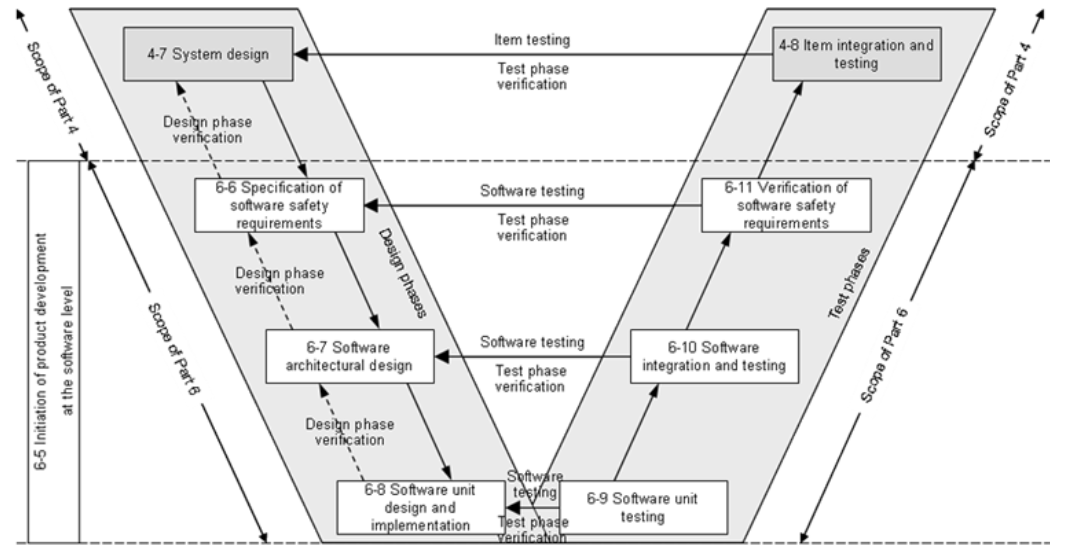
\includegraphics[keepaspectratio, width=\linewidth]{pictures/V}
  \label{IMG:phase_model}
  \caption{Phase model for software development}
\end{figure}

The first step is the system design. At this point the system specification is
written, and then the software specifications. When all specifications exists,
the next phase is to design the software architecture. The last part of the
design is software unit design and implementation. All phases must be a
verification of the former phase.

When the implementation is done, it is time for the test phases. These begins
with software unit testing which tests the software unit design phase. If the
tests verifies that the software unit design and implementation is correct, the
test phase moves on to the architectural design and then to verification of
software safety requirements.
The last test phase verifies that the system is
designed according to the specification. %It is important that the test phases
%test the specifications and not the
%implementation.

%Aim for the work. What should be accomplished?
\section{Purpose}
The purpose is to automate the testing process in an effective and good way.
To make it possible to raise the Automotive Safety Integration Level (ASIL), in
the software unit design and implementation phase and in the software %% n�mner
 %% ASIL utan att ha pratat om det tidigare.
architectural design phase, a check must be done to see if it exist a tool that
can be used in order to perform a semi formal verification of a module, and
then make this process generalized for modules in coexistence.\\ %% v�ldigt l�ng
 %% mening

The purpose is also to be able to decrease the number of needed unit tests in
the software unit design and implementation phase. Even further is the goal to
introduce semi formal verification of the software architectural design phase.
The functional safety concept will be most important in this phase.

%question formulation?
%The problem at hand, the assignment
\section{Objective}
The objective is to propose and motivate what should be done to be able to
achieve a semi formal verification. This should include a confidence interval
for how certain the verification is.

The objective is also to prove that it is possible to do semi formal
verification for an AUTOSAR module and its specification. This should be
generalized so its possible to test other specifications and modules at a later
moment. It should also not matter which configuration that is active, because
the specification should hold for all configurations.

%Limitations. What should be left out and why?
\section{Scope}
We will use AUTOSAR 4.0 revision 3 for our thesis work.
Since this version of AUTOSAR consists of around 80 specifications and other
auxiliary materials \cite{AUTOSAR:URL}, we will limit our scope to one or two
specifications. The main module of this thesis is the CryptoServiceManager. This
module provides cryptographic functionalities for synchronous and asynchronous
services. This module is chosen because it only got a few dependencies, is used
%% "is used to trace development and production errors"?
to trace development and production errors but also to incorporate cryptographic
libraries.

It is hard to test that a call to another module gives the right results. This
is the reason why we have chosen a module with a small number of
dependencies. The CryptoServiceManager should also have functionality which
gives the same results no matter which state it is in, such as hash
functions \cite{SPEC:AUTOSAR:CSM}. %% f�rklara varf�r detta �r bra.

Also the aim of the work is to verify software components. In other words no
work considered hardware or a combination of hardware and software will be
prioritized. All implemented code for the verification will run on a standard
PC-machine.

%% l�gga till ett stycke ang�ende att vi bara g�r in p� 6-9 och 6-10, och inte
%% p� 6-8 eller 6-11.


%Method of accomplishment. How should the work be carried out?
\chapter{Method}
%% kolla att allt �r i imperfekt
%% verb i passiv form

\section{Choose of tool for verification}
Software unit testing can be achieved by almost any tool.
%% motivera.
Consequently this phase is not the most interesting when it comes to the choose
of a tool verification. Of course one can take the simplicity to achieve good
%% "simplicity" - av vad?
unit testing into account, but still it is not what makes a verification tool
especially unique for the project goals.

Since the purpose is about benchmarking software the phase ''verification of
software safety requirements'' will not influence the choose. To be able to test
this phase, a greater amount of components of the whole system must be
available. Such components may include hardware etcetera. Implementation wise
%% "etcetera" borde arbetas bort.
should everything be able to run on a standard PC-machine.

The most interesting part is the software integration and testing. Is there a
tool that one can use to easily combine test and requirements from different
modules? Is it possible to test functional safety concept from this
combination, for example by corrupting some software elements?

%\subsection{Why QuickCheck and Erlang?}

\section{Specification}
In AUTOSAR, specifications for each module is given in text form. Consequently
one must first, before a module can be tested, implement the specification for
that module in code.

\section{Testing}
%% vilka properties? quickcheck?
%% kanske �r b�ttre att skriva "Module properties have to take..."
%% alternativt "Quickcheck properties for a module have to take..."
Properties for a module have to take the current state in consideration, since
most functions written in an imperative language are not immutable. This gives
raise to the idea of a state based testing tool.
%% .. och pl�tsligt: en lista:...
\begin{itemize}
\item Choose a specification which will be translated to QuickCheck properties
in parts.
\item With the use of statistics and confidence intervals, show that, with
enough tests the state-space will be exhausted.
\item Evaluate other semi formal techniques and show that the results from them
shows that QuickCheck is reliable for verification.
\item Generalize the technique.
\end{itemize}

\section{Implementation}
A challenging step is the analysis of the results. If the testing tool returns zero
errors what does that say about the robustness of the input byte code? Passed
100 of 100 tests is just a statement and does not say anything more than that
some tests passed. Can tests be implemented in a clever way so that it is
possible to get some kind of confidence interval on the correctness of the code?

\begin{figure}[!ht]
% Graphic for TeX using PGF
% Title: /home/oskar/documents/box.dia
% Creator: Dia v0.97.2
% CreationDate: Sat Sep  7 19:28:43 2013
% For: oskar
% \usepackage{tikz}
% The following commands are not supported in PSTricks at present
% We define them conditionally, so when they are implemented,
% this pgf file will use them.
\ifx\du\undefined
  \newlength{\du}
\fi
\setlength{\du}{15\unitlength}
\begin{tikzpicture}
\pgftransformxscale{1.000000}
\pgftransformyscale{-1.000000}
\definecolor{dialinecolor}{rgb}{0.000000, 0.000000, 0.000000}
\pgfsetstrokecolor{dialinecolor}
\definecolor{dialinecolor}{rgb}{1.000000, 1.000000, 1.000000}
\pgfsetfillcolor{dialinecolor}
\definecolor{dialinecolor}{rgb}{1.000000, 1.000000, 1.000000}
\pgfsetfillcolor{dialinecolor}
\fill (6.000000\du,7.000000\du)--(6.000000\du,11.000000\du)--(10.795000\du,11.000000\du)--(10.795000\du,7.000000\du)--cycle;
\pgfsetlinewidth{0.100000\du}
\pgfsetdash{}{0pt}
\pgfsetdash{}{0pt}
\pgfsetmiterjoin
\definecolor{dialinecolor}{rgb}{0.000000, 0.000000, 0.000000}
\pgfsetstrokecolor{dialinecolor}
\draw (6.000000\du,7.000000\du)--(6.000000\du,11.000000\du)--(10.795000\du,11.000000\du)--(10.795000\du,7.000000\du)--cycle;
% setfont left to latex
\definecolor{dialinecolor}{rgb}{0.000000, 0.000000, 0.000000}
\pgfsetstrokecolor{dialinecolor}
\node at (8.397500\du,9.195000\du){Testing Tool};
\pgfsetlinewidth{0.100000\du}
\pgfsetdash{}{0pt}
\pgfsetdash{}{0pt}
\pgfsetbuttcap
{
\definecolor{dialinecolor}{rgb}{0.000000, 0.000000, 0.000000}
\pgfsetfillcolor{dialinecolor}
% was here!!!
\pgfsetarrowsend{stealth}
\definecolor{dialinecolor}{rgb}{0.000000, 0.000000, 0.000000}
\pgfsetstrokecolor{dialinecolor}
\draw (10.795000\du,9.000000\du)--(12.000000\du,9.050000\du);
}
\pgfsetlinewidth{0.100000\du}
\pgfsetdash{}{0pt}
\pgfsetdash{}{0pt}
\pgfsetbuttcap
{
\definecolor{dialinecolor}{rgb}{0.000000, 0.000000, 0.000000}
\pgfsetfillcolor{dialinecolor}
% was here!!!
\pgfsetarrowsend{stealth}
\definecolor{dialinecolor}{rgb}{0.000000, 0.000000, 0.000000}
\pgfsetstrokecolor{dialinecolor}
\draw (0.000000\du,9.000000\du)--(6.000000\du,9.000000\du);
}
% setfont left to latex
\definecolor{dialinecolor}{rgb}{0.000000, 0.000000, 0.000000}
\pgfsetstrokecolor{dialinecolor}
\node[anchor=west] at (8.397500\du,9.000000\du){};
% setfont left to latex
\definecolor{dialinecolor}{rgb}{0.000000, 0.000000, 0.000000}
\pgfsetstrokecolor{dialinecolor}
\node[anchor=west] at (0.000000\du,10.000000\du){Module byte code};
% setfont left to latex
\definecolor{dialinecolor}{rgb}{0.000000, 0.000000, 0.000000}
\pgfsetstrokecolor{dialinecolor}
\node[anchor=west] at (3.000000\du,8.000000\du){};
% setfont left to latex
\definecolor{dialinecolor}{rgb}{0.000000, 0.000000, 0.000000}
\pgfsetstrokecolor{dialinecolor}
\node[anchor=west] at (2.000000\du,5.000000\du){Module specfication};
\definecolor{dialinecolor}{rgb}{1.000000, 1.000000, 1.000000}
\pgfsetfillcolor{dialinecolor}
\fill (12.000000\du,7.000000\du)--(12.000000\du,11.100000\du)--(17.800000\du,11.100000\du)--(17.800000\du,7.000000\du)--cycle;
\pgfsetlinewidth{0.100000\du}
\pgfsetdash{}{0pt}
\pgfsetdash{}{0pt}
\pgfsetmiterjoin
\definecolor{dialinecolor}{rgb}{0.000000, 0.000000, 0.000000}
\pgfsetstrokecolor{dialinecolor}
\draw (12.000000\du,7.000000\du)--(12.000000\du,11.100000\du)--(17.800000\du,11.100000\du)--(17.800000\du,7.000000\du)--cycle;
% setfont left to latex
\definecolor{dialinecolor}{rgb}{0.000000, 0.000000, 0.000000}
\pgfsetstrokecolor{dialinecolor}
\node at (14.900000\du,9.245000\du){};
\pgfsetlinewidth{0.100000\du}
\pgfsetdash{}{0pt}
\pgfsetdash{}{0pt}
\pgfsetmiterjoin
\pgfsetbuttcap
{
\definecolor{dialinecolor}{rgb}{0.000000, 0.000000, 0.000000}
\pgfsetfillcolor{dialinecolor}
% was here!!!
\pgfsetarrowsend{stealth}
{\pgfsetcornersarced{\pgfpoint{0.000000\du}{0.000000\du}}\definecolor{dialinecolor}{rgb}{0.000000, 0.000000, 0.000000}
\pgfsetstrokecolor{dialinecolor}
\draw (1.000000\du,5.000000\du)--(1.000000\du,6.000000\du)--(8.000000\du,6.000000\du)--(8.000000\du,7.000000\du);
}}
% setfont left to latex
\definecolor{dialinecolor}{rgb}{0.000000, 0.000000, 0.000000}
\pgfsetstrokecolor{dialinecolor}
\node at (14.900000\du,9.050000\du){Output};
% setfont left to latex
\definecolor{dialinecolor}{rgb}{0.000000, 0.000000, 0.000000}
\pgfsetstrokecolor{dialinecolor}
\node at (14.900000\du,9.850000\du){ analysis };
\end{tikzpicture}

\caption{Abstract implementation module}
\end{figure}

%Gantt-schema.
\chapter{Time-plan}
\section{Provisional plan}
Exactly how things should be done isn't clear. Therefor we are proposing a more
orderly plan to be able learn what can be done and where problems may lie a
head. At first just try to implement one or two simple rules from an AUTOSAR
specification, in Erlang, and try to run it on AUTOSAR module. It's important to
notice that this may have nothing to do with our final solution and is mostly
for evaluating what can be done in QuickCheck. Since our work is not just about
implementing tests, but rather show that we can make semi formal verification on
a module in AUTOSAR, the number of rules that we implement seems less relevant
than what we can do with the rules that we implement.

The next step is to analyse the results and come to a conclusion for how to
continue. Possible Erlang and QuickCheck is not suited for our goals.
More information about this can be found on the Gantt scheme
represented below.

\begin{ganttchart}[vgrid={dotted}, today=9, today label={Current week}, today offset=.5]{1}{20}
  \setganttlinklabel{s-s}{}
  \setganttlinklabel{f-s}{}
  \gantttitle{2013}{17}\gantttitle{2014}{3} \\
  \gantttitlelist{36,...,52,1,2,3}{1} \\
  %\ganttgroup{Group 1}{1}{10} \\
  \ganttbar[name=planning]{Planning}{1}{2} \\
  \ganttbar[name=research]{Research}{2}{5}\\
  \ganttbar[name=semiformal]{Semi formal verification}{2}{5}\\
%  \ganttgroup[inline, group top shift=1.1, group left shift=0.4, group label font=\normalsize, group height=0.1]{Course}{2}{8}\\
  \ganttbar[name=course]{QuviQ Erlang course}{8}{9}\\
  \ganttbar[name=analysis]{Analysis of other tools}{2}{3}\\
  \ganttbar[name=decision]{Decision of technique}{4}{4} \\
  \ganttbar[name=firsttest]{First test}{5}{6}\\
  \ganttbar[name=implementation]{Implementation}{8}{11} \\
  \ganttbar[name=evaluation]{Evaluation of results}{12}{13}\\
  \ganttbar[name=focus]{Focus on thesis}{14}{15}\\
  \ganttmilestone[name=mecel]{Presentation to Mecel}{16}\\
  \ganttbar[name=polish]{Polish}{17}{20}\\
  \ganttbar[name=opposition]{Opposition}{17}{20}\\
  \ganttmilestone[name=chalmers]{Presentation to Chalmers}{20}\\
  \ganttbar{Thesis}{1}{20}
  \ganttlink{semiformal}{course} % semi formal - erlang course
  \ganttlink[link type=f-s]{firsttest}{course} % erlang course - first test
  \ganttlink[link type=f-s]{analysis}{decision} % other tools - first test
  \ganttlink[link type=f-s]{decision}{firsttest} % first test - other tools (end)
  \ganttlink[link type=f-s]{firsttest}{implementation} % decision - implementation
  \ganttlink[link type=f-s]{implementation}{evaluation} % implementation - evaluation
%  \ganttlink[link type=f-s]{evaluation}{focus} % evaluation - focus on thesis
  \ganttlink{focus}{mecel} % focus on thesis - presentation to mecel
\end{ganttchart}

Finding out the exact definition of semi formal verification and getting an idea of how this
can be implemented is a fundamental step. Hence this is added explicitly, as
shown in the Gantt Scheme, to the project plan.
In the first test week we translate some specification
demands to QuickCheck code, and test if it is possible to prove that this is
semi formal verfied. The purpose of doing analysis of other tools is to see if there exists better
tools for our goals, we should then decide which tools and techniques to use.
A presentation to Mecel is planned to the last week in December.  In January we
present our work to Chalmers.


\bibliographystyle{vancouver}
\bibliography{references}


\end{document}
